\documentclass[12pt]{article}
\usepackage[utf8]{inputenc}
\usepackage{amsmath, amssymb}
\usepackage{xcolor}
\usepackage{geometry}
\usepackage{hyperref}
\usepackage{fancyhdr}
\usepackage{enumitem}
\usepackage{minted} % Code highlighting
\usepackage{booktabs} % Clean tables
\usepackage{tikz}
\usetikzlibrary{shapes, arrows, positioning, automata}

\geometry{margin=1in}
\hypersetup{colorlinks=true, linkcolor=blue, urlcolor=cyan}

\pagestyle{fancy}
\fancyhf{}
\fancyhead[L]{\textbf{\TOPICTITLE}}
\fancyhead[R]{\thepage}

% -------------------------------
% Topic Metadata
% -------------------------------
\newcommand{\TOPICTITLE}{Principles of Reliable Data Transfer}
\title{\TOPICTITLE\\\large Study-Ready Notes}
\author{Compiled by Andrew Photinakis}
\date{\today}

\setlength{\headheight}{15pt}

\begin{document}
\maketitle
\tableofcontents
\newpage

% This LaTeX file should be saved at: computer_networks/transport_layer/principles_reliable_data_transfer.tex

\section{Introduction to Reliable Data Transfer}

\begin{itemize}
    \item Core component of transport-layer services
    \item Essential for connection-oriented protocols like TCP
    \item Builds upon multiplexing/demultiplexing concepts
    \item Addresses challenges of unreliable network channels
\end{itemize}

\textcolor{blue}{[Summary: Reliable data transfer protocols ensure data delivery despite unreliable network conditions, using mechanisms like acknowledgments, sequence numbers, and retransmissions.]}

\section{Reliable Data Transfer Service Abstraction}

\subsection{Service Model}
\begin{itemize}
    \item \textbf{Abstraction}: Perfectly reliable channel between sending and receiving processes
    \item \textbf{Reality}: Underlying channel is unreliable (loses, corrupts, reorders data)
    \item \textbf{Implementation}: Transport layer protocols handle reliability
\end{itemize}

\begin{figure}[h]
    \centering
    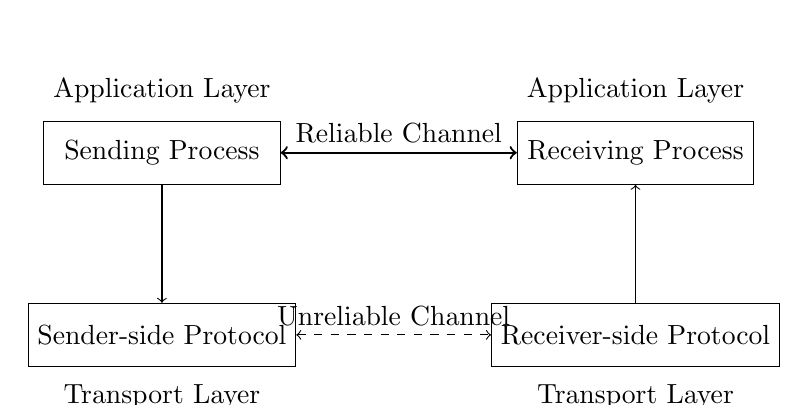
\begin{tikzpicture}[
            node distance=1.5cm,
            proc/.style={rectangle, draw, minimum width=3cm, minimum height=0.8cm}
        ]
        % Ideal abstraction
        \node[proc] (send1) {Sending Process};
        \node[proc, right=3cm of send1] (recv1) {Receiving Process};
        \draw[<->, thick] (send1) -- node[above] {Reliable Channel} (recv1);

        % Actual implementation
        \node[proc, below=1.5cm of send1] (send2) {Sender-side Protocol};
        \node[proc, below=1.5cm of recv1] (recv2) {Receiver-side Protocol};
        \draw[<->, dashed] (send2) -- node[above] {Unreliable Channel} (recv2);

        % Connections
        \draw[->] (send1) -- (send2);
        \draw[->] (recv2) -- (recv1);

        % Labels
        \node[above=0.1cm of send1] {Application Layer};
        \node[above=0.1cm of recv1] {Application Layer};
        \node[below=0.1cm of send2] {Transport Layer};
        \node[below=0.1cm of recv2] {Transport Layer};

    \end{tikzpicture}
    \caption{Reliable data transfer: abstraction vs implementation}
    \label{fig:rdt_abstraction}
\end{figure}

\section{RDT Protocol Interfaces and Mechanisms}

\subsection{Protocol Interface Functions}
\begin{itemize}
    \item \textbf{rdt\_send()}: Called from above to deliver data to receiver upper layer
    \item \textbf{udt\_send()}: Called by RDT to transfer packet over unreliable channel
    \item \textbf{rdt\_rcv()}: Called when packet arrives on receiver side
    \item \textbf{deliver\_data()}: Called by RDT to deliver data to upper layer
\end{itemize}

\subsection{Key Protocol Mechanisms}
\begin{itemize}
    \item Error detection (checksums)
    \item Acknowledgments (ACKs) and Negative Acknowledgments (NAKs)
    \item Retransmission
    \item Sequence numbers for duplicate detection
    \item Timers for loss detection
\end{itemize}

\textcolor{orange}{[Mnemonic: "ACE RT" - Acknowledgments, Checksums, Error detection, Retransmission, Timers - key RDT mechanisms.]}

\section{Finite State Machine Specification}

\subsection{FSM Concepts}
\begin{itemize}
    \item Used to specify sender and receiver behavior
    \item \textbf{State}: Current condition of protocol entity
    \item \textbf{Event}: Trigger that may cause state transition
    \item \textbf{Actions}: Operations performed during transition
\end{itemize}

\begin{figure}[h]
    \centering
    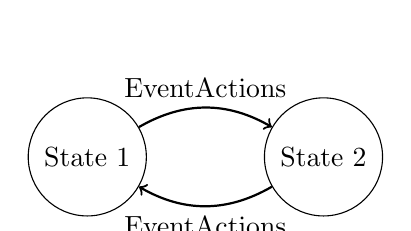
\begin{tikzpicture}[
            node distance=3cm,
            state/.style={circle, draw, minimum size=1.5cm}
        ]
        \node[state] (state1) {State 1};
        \node[state, right of=state1] (state2) {State 2};

        \draw[->, thick] (state1) to[bend left] node[above] {Event \\ Actions} (state2);
        \draw[->, thick] (state2) to[bend left] node[below] {Event \\ Actions} (state1);

    \end{tikzpicture}
    \caption{Finite State Machine basic structure}
    \label{fig:fsm_basic}
\end{figure}

\section{RDT1.0: Reliable Transfer over Reliable Channel}

\subsection{Assumptions}
\begin{itemize}
    \item Underlying channel is perfectly reliable
    \item No bit errors
    \item No loss of packets
\end{itemize}

\subsection{FSM Specifications}
\begin{figure}[h]
    \centering
    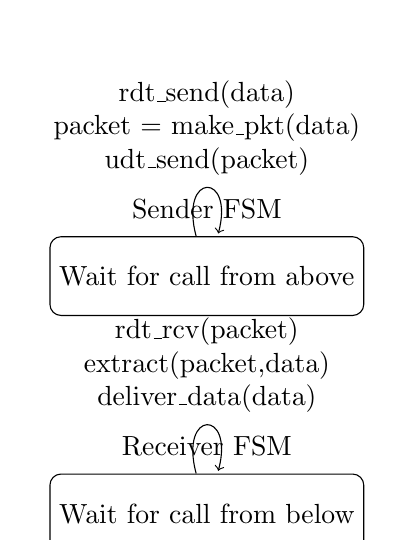
\begin{tikzpicture}[
            node distance=3cm,
            state/.style={rectangle, draw, rounded corners, minimum width=2.5cm, minimum height=1cm}
        ]
        % Sender FSM
        \node[state] (send_wait) {Wait for call from above};
        \path[->] (send_wait) edge[loop above] node {
                \begin{tabular}{c}
                    rdt\_send(data)          \\
                    packet = make\_pkt(data) \\
                    udt\_send(packet)
                \end{tabular}
            } ();

        % Receiver FSM
        \node[state, below=2cm of send_wait] (recv_wait) {Wait for call from below};
        \path[->] (recv_wait) edge[loop above] node {
                \begin{tabular}{c}
                    rdt\_rcv(packet)     \\
                    extract(packet,data) \\
                    deliver\_data(data)
                \end{tabular}
            } ();

        \node[above=0.1cm of send_wait] {Sender FSM};
        \node[above=0.1cm of recv_wait] {Receiver FSM};
    \end{tikzpicture}
    \caption{RDT1.0: Simple FSMs for perfectly reliable channel}
    \label{fig:rdt1_fsm}
\end{figure}

\textcolor{blue}{[Summary: RDT1.0 assumes perfect channel conditions - sender simply sends packets, receiver simply receives and delivers them without error handling.]}

\section{RDT2.0: Channel with Bit Errors}

\subsection{New Challenges}
\begin{itemize}
    \item Underlying channel may flip bits in packets
    \item Use checksums to detect bit errors
    \item Recovery mechanisms needed
\end{itemize}

\subsection{Error Recovery Mechanisms}
\begin{itemize}
    \item \textbf{Acknowledgments (ACKs)}: Receiver tells sender packet received OK
    \item \textbf{Negative Acknowledgments (NAKs)}: Receiver tells sender packet had errors
    \item \textbf{Stop-and-wait}: Sender sends one packet, waits for receiver response
\end{itemize}

\begin{figure}[h]
    \centering
    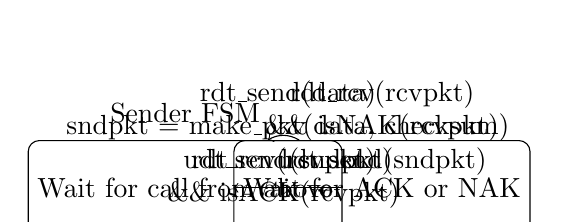
\begin{tikzpicture}[
            node distance=2.5cm,
            state/.style={rectangle, draw, rounded corners, minimum width=2.8cm, minimum height=1.2cm}
        ]
        % Sender FSM
        \node[state] (send_wait_call) {Wait for call from above};
        \node[state, right of=send_wait_call] (send_wait_ack) {Wait for ACK or NAK};

        \draw[->] (send_wait_call) -- node[above] {
            \begin{tabular}{c}
                rdt\_send(data)                    \\
                sndpkt = make\_pkt(data, checksum) \\
                udt\_send(sndpkt)
            \end{tabular}
        } (send_wait_ack);

        \draw[->] (send_wait_ack) to[bend left] node[above] {
            \begin{tabular}{c}
                rdt\_rcv(rcvpkt)   \\
                \&\& isNAK(rcvpkt) \\
                udt\_send(sndpkt)
            \end{tabular}
        } (send_wait_ack);

        \draw[->] (send_wait_ack) to[bend right] node[below] {
            \begin{tabular}{c}
                rdt\_rcv(rcvpkt) \\
                \&\& isACK(rcvpkt)
            \end{tabular}
        } (send_wait_call);

        \node[above=0.1cm of send_wait_call] {Sender FSM};
    \end{tikzpicture}
    \caption{RDT2.0 sender FSM handling bit errors}
    \label{fig:rdt2_sender}
\end{figure}

\section{RDT2.1: Handling Garbled ACK/NAKs}

\subsection{The Fatal Flaw in RDT2.0}
\begin{itemize}
    \item What if ACK/NAK becomes corrupted?
    \item Sender doesn't know what happened at receiver
    \item Can't just retransmit: possible duplicate
\end{itemize}

\subsection{Solution: Sequence Numbers}
\begin{itemize}
    \item Add sequence number to each packet
    \item Two sequence numbers (0,1) suffice for stop-and-wait
    \item Receiver discards duplicate packets
\end{itemize}

\textcolor{teal}{[Concept Map: RDT Evolution → RDT1.0 (perfect channel) → RDT2.0 (bit errors, ACK/NAK) → RDT2.1 (garbled ACKs, sequence numbers) → Each version adds mechanisms to handle more realistic channel impairments.]}

\section{RDT2.2: NAK-Free Protocol}

\subsection{Approach}
\begin{itemize}
    \item Same functionality as RDT2.1 but using ACKs only
    \item Instead of NAK, receiver sends ACK for last packet received OK
    \item Receiver explicitly includes sequence number of packet being ACKed
    \item Duplicate ACK at sender triggers retransmission (same as NAK)
\end{itemize}

\begin{table}[h]
    \centering
    \begin{tabular}{p{0.45\textwidth}p{0.45\textwidth}}
        \toprule
        \textbf{RDT2.1 (with NAKs)}              & \textbf{RDT2.2 (NAK-free)}              \\
        \midrule
        Uses ACK and NAK messages                & Uses only ACK messages                  \\
        Receiver sends NAK for corrupted packets & Receiver sends ACK for last good packet \\
        Simpler logic                            & Reduced message types                   \\
        Two response types                       & Unified response mechanism              \\
        \textbf{Used in}: Educational examples   & \textbf{Used in}: TCP (real-world)      \\
        \bottomrule
    \end{tabular}
    \caption{Comparison of RDT2.1 vs RDT2.2}
    \label{tab:rdt21_vs_rdt22}
\end{table}

\section{RDT3.0: Channels with Errors and Loss}

\subsection{New Channel Assumptions}
\begin{itemize}
    \item Underlying channel can lose packets (data and ACKs)
    \item Need mechanism to detect and recover from lost packets
\end{itemize}

\subsection{Solution: Countdown Timer}
\begin{itemize}
    \item Sender waits "reasonable" amount of time for ACK
    \item Retransmits if no ACK received in this time
    \item If packet just delayed (not lost): retransmission creates duplicate
    \item Sequence numbers handle duplicates
\end{itemize}

\begin{figure}[h]
    \centering
    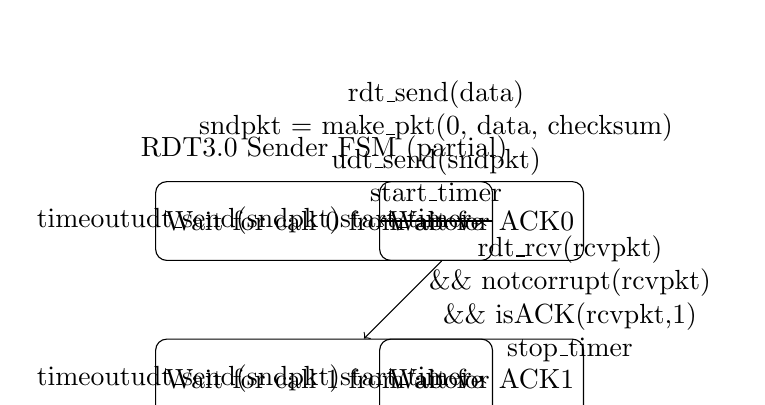
\begin{tikzpicture}[
            node distance=2cm,
            state/.style={rectangle, draw, rounded corners, minimum width=2.5cm, minimum height=1cm}
        ]
        \node[state] (wait0) {Wait for call 0 from above};
        \node[state, right of=wait0] (wait_ack0) {Wait for ACK0};
        \node[state, below of=wait0] (wait1) {Wait for call 1 from above};
        \node[state, right of=wait1] (wait_ack1) {Wait for ACK1};

        % Transitions from wait0
        \draw[->] (wait0) -- node[above] {
            \begin{tabular}{c}
                rdt\_send(data)                       \\
                sndpkt = make\_pkt(0, data, checksum) \\
                udt\_send(sndpkt)                     \\
                start\_timer
            \end{tabular}
        } (wait_ack0);

        % Timer transitions
        \draw[->] (wait_ack0) to[bend right] node[left] {timeout \\ udt\_send(sndpkt) \\ start\_timer} (wait_ack0);
        \draw[->] (wait_ack1) to[bend right] node[left] {timeout \\ udt\_send(sndpkt) \\ start\_timer} (wait_ack1);

        % ACK transitions
        \draw[->] (wait_ack0) -- node[right] {
            \begin{tabular}{c}
                rdt\_rcv(rcvpkt)        \\
                \&\& notcorrupt(rcvpkt) \\
                \&\& isACK(rcvpkt,1)    \\
                stop\_timer
            \end{tabular}
        } (wait1);

        \node[above=0.1cm of wait0] {RDT3.0 Sender FSM (partial)};
    \end{tikzpicture}
    \caption{RDT3.0 sender with timer for loss recovery}
    \label{fig:rdt3_sender}
\end{figure}

\section{RDT3.0 Operation Scenarios}

\subsection{Four Key Scenarios}
\begin{enumerate}
    \item \textbf{No loss}: Normal operation with timely ACKs
    \item \textbf{Packet loss}: Timeout triggers retransmission
    \item \textbf{ACK loss}: Duplicate ACK triggers retransmission
    \item \textbf{Premature timeout}: Delayed ACK causes unnecessary retransmission
\end{enumerate}

\begin{table}[h]
    \centering
    \begin{tabular}{p{0.22\textwidth}p{0.35\textwidth}p{0.35\textwidth}}
        \toprule
        \textbf{Scenario} & \textbf{Problem}            & \textbf{Solution}                 \\
        \midrule
        No loss           & None                        & Normal operation                  \\
        Packet loss       & Data packet lost in transit & Timeout and retransmission        \\
        ACK loss          & Acknowledgment lost         & Timeout and retransmission        \\
        Premature timeout & ACK delayed, not lost       & Sequence numbers handle duplicate \\
        \bottomrule
    \end{tabular}
    \caption{RDT3.0 operation scenarios and solutions}
    \label{tab:rdt3_scenarios}
\end{table}

\textcolor{blue}{[Summary: RDT3.0 handles both bit errors and packet loss using checksums, sequence numbers, acknowledgments, and countdown timers, providing complete reliability over unreliable channels.]}

\section{Performance Analysis of RDT3.0}

\subsection{Sender Utilization}
\begin{itemize}
    \item \textbf{U\_sender}: Fraction of time sender is busy sending
    \item For stop-and-wait protocol: very low utilization
\end{itemize}

\subsection{Utilization Formula}
\[
    U_{sender} = \frac{L/R}{RTT + L/R}
\]

Where:
\begin{itemize}
    \item $L$ = packet length (bits)
    \item $R$ = transmission rate (bps)
    \item $RTT$ = round-trip time
\end{itemize}

\subsection{Example Calculation}
\begin{itemize}
    \item 1 Gbps link, 15 ms propagation delay, 8000 bit packet
    \item Transmission time: $D_{trans} = \frac{L}{R} = \frac{8000}{10^9} = 8$ microseconds
    \item $RTT = 2 \times 15$ ms = 30 ms
    \item $U_{sender} = \frac{0.008}{30.008} = 0.00027$
\end{itemize}

\textcolor{orange}{[Mnemonic: "Low Utilization Long Wait" - Stop-and-wait protocols have low utilization due to waiting for ACKs.]}

\section{Pipelined Protocols}

\subsection{Limitations of Stop-and-Wait}
\begin{itemize}
    \item Very low utilization (0.027\% in example)
    \item Protocol limits performance of underlying infrastructure
    \item Most of the time, sender is idle waiting for ACK
\end{itemize}

\subsection{Pipelining Solution}
\begin{itemize}
    \item Allow multiple "in-flight" packets
    \item Increase range of sequence numbers
    \item Require buffering at sender and/or receiver
    \item Dramatically increases utilization
\end{itemize}

\subsection{Utilization with Pipelining}
\[
    U_{sender} = \frac{N \times L/R}{RTT + L/R}
\]
Where $N$ is the number of pipelined packets.

\begin{figure}[h]
    \centering
    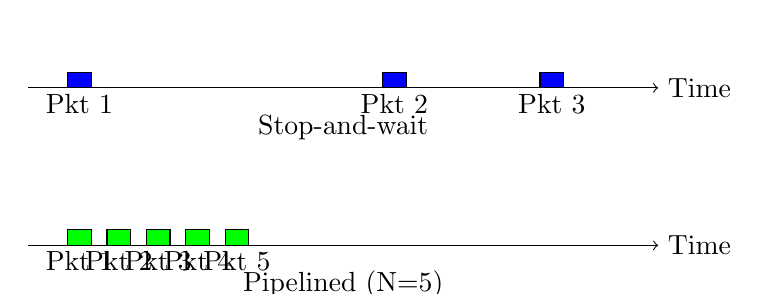
\begin{tikzpicture}
        % Timeline without pipelining
        \draw[->] (0,2) -- (8,2) node[right] {Time};
        \foreach \x/\y in {0.5/1, 4.5/2, 6.5/3} {
                \draw[fill=blue] (\x,2) rectangle (\x+0.3,2.2);
                \node at (\x+0.15,1.8) {Pkt \y};
            }
        \node at (4,1.5) {Stop-and-wait};

        % Timeline with pipelining
        \draw[->] (0,0) -- (8,0) node[right] {Time};
        \foreach \x/\y in {0.5/1, 1.0/2, 1.5/3, 2.0/4, 2.5/5} {
                \draw[fill=green] (\x,0) rectangle (\x+0.3,0.2);
                \node at (\x+0.15,-0.2) {Pkt \y};
            }
        \node at (4,-0.5) {Pipelined (N=5)};
    \end{tikzpicture}
    \caption{Comparison of stop-and-wait vs pipelined transmission}
    \label{fig:pipelining_comparison}
\end{figure}

\section{Go-Back-N Protocol}

\subsection{Sender Operation}
\begin{itemize}
    \item Window of up to N consecutive transmitted but unACKed packets
    \item k-bit sequence number in packet header
    \item \textbf{Cumulative ACK}: ACK(n) acknowledges all packets up to and including sequence number n
    \item Single timer for oldest in-flight packet
    \item Timeout(n): retransmit packet n and all higher sequence number packets in window
\end{itemize}

\subsection{Sender Window Structure}
\begin{figure}[h]
    \centering
    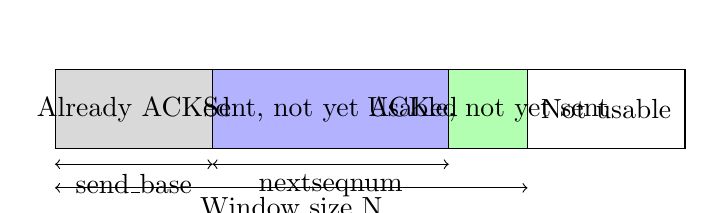
\begin{tikzpicture}
        \draw (0,0) rectangle (8,1);
        \draw[fill=gray!30] (0,0) rectangle (2,1);
        \draw[fill=blue!30] (2,0) rectangle (5,1);
        \draw[fill=green!30] (5,0) rectangle (6,1);
        \draw (6,0) -- (6,1);

        \node at (1,0.5) {Already ACKed};
        \node at (3.5,0.5) {Sent, not yet ACKed};
        \node at (5.5,0.5) {Usable, not yet sent};
        \node at (7,0.5) {Not usable};

        \draw[<->] (0,-0.2) -- node[below] {send\_base} (2,-0.2);
        \draw[<->] (2,-0.2) -- node[below] {nextseqnum} (5,-0.2);
        \draw[<->] (0,-0.5) -- node[below] {Window size N} (6,-0.5);
    \end{tikzpicture}
    \caption{Go-Back-N sender window structure}
    \label{fig:gbn_window}
\end{figure}

\section{Selective Repeat Protocol}

\subsection{Key Features}
\begin{itemize}
    \item Receiver individually acknowledges all correctly received packets
    \item Buffers out-of-order packets for eventual in-order delivery
    \item Sender maintains timer for each unACKed packet
    \item More efficient but more complex than Go-Back-N
\end{itemize}

\subsection{Window Size Constraint}
\begin{itemize}
    \item Critical relationship between sequence number space and window size
    \item For sequence numbers 0 to $2^k - 1$, window size must satisfy:
          \[
              N \leq 2^{k-1}
          \]
    \item Prevents ambiguity between old and new packets
\end{itemize}

\begin{table}[h]
    \centering
    \begin{tabular}{p{0.45\textwidth}p{0.45\textwidth}}
        \toprule
        \textbf{Go-Back-N}            & \textbf{Selective Repeat}    \\
        \midrule
        Cumulative acknowledgments    & Individual acknowledgments   \\
        Discards out-of-order packets & Buffers out-of-order packets \\
        Single timer for window       & Timer per packet             \\
        Simpler implementation        & More complex implementation  \\
        Less efficient with loss      & More efficient with loss     \\
        Window: $N \leq 2^k - 1$      & Window: $N \leq 2^{k-1}$     \\
        \bottomrule
    \end{tabular}
    \caption{Comparison of Go-Back-N vs Selective Repeat}
    \label{tab:gbn_vs_sr}
\end{table}

\textcolor{teal}{[Concept Map: Pipelined Protocols → Go-Back-N (cumulative ACKs, simple) vs Selective Repeat (individual ACKs, efficient) → Trade-off between complexity and performance → Window size constraints critical for correctness.]}

\section{Study Aids and Exam Preparation}

\subsection{Key Concepts to Master}
\begin{itemize}
    \item Understand the evolution of RDT protocols and what problem each version solves
    \item Be able to draw and interpret FSM diagrams for each protocol version
    \item Calculate sender utilization for stop-and-wait and pipelined protocols
    \item Explain the window size constraints for Go-Back-N and Selective Repeat
    \item Compare and contrast different reliability mechanisms
\end{itemize}

\subsection{Practice Questions}
\begin{enumerate}
    \item \textbf{Trace the evolution} of RDT protocols from 1.0 to 3.0. What specific problem does each new version address, and what mechanism does it introduce?

    \item Calculate the \textbf{sender utilization} for a stop-and-wait protocol with the following parameters: packet size = 1500 bytes, transmission rate = 100 Mbps, RTT = 50 ms. How does this change if we use pipelining with a window size of 10?

    \item Explain why \textbf{Selective Repeat} requires that the window size be at most half the sequence number space, while \textbf{Go-Back-N} can use almost the entire sequence number space.

    \item Draw the \textbf{FSM for RDT3.0 sender} and explain how it handles packet loss, ACK loss, and premature timeouts.

    \item Compare the \textbf{performance characteristics} of Go-Back-N vs Selective Repeat in a network with high packet loss rates. Which would you choose and why?
\end{enumerate}

\textcolor{orange}{[Mnemonic: "RDT 1-2-3" - RDT1.0 (perfect), RDT2.0 (errors), RDT3.0 (loss) - each adds one more real-world problem to solve.]}

\section{Summary}

\begin{itemize}
    \item Reliable data transfer protocols build reliability over unreliable channels
    \item Key mechanisms: error detection, acknowledgments, sequence numbers, timers, retransmissions
    \item RDT protocol evolution addresses increasingly realistic channel impairments
    \item Stop-and-wait protocols have poor utilization; pipelining dramatically improves performance
    \item Go-Back-N and Selective Repeat are two pipelined approaches with different trade-offs
    \item Window size constraints are critical for protocol correctness
\end{itemize}

\end{document}